
%(BEGIN_QUESTION)
% Copyright 2010, Tony R. Kuphaldt, released under the Creative Commons Attribution License (v 1.0)
% This means you may do almost anything with this work of mine, so long as you give me proper credit

Examine this P\&ID for a temperature-controlled fermenting vessel used in a brewery, where liquid {\it glycol} is chilled to a low temperature of 4 degrees Celsius and then used as a coolant to remove heat energy from the batch inside the fermenter through a {\it jacket} on the fermenting vessel, maintaining it at a temperature below ambient:

$$\includegraphics[width=15.5cm]{i03397x01.eps}$$

Suppose the temperature controller (TRC-125) is configured for {\it proportional-only control}, and it happens to be maintaining the brew temperature at a setpoint of 5$^{o}$ C.  Now suppose the operator increases the setpoint in two equal steps to 15$^{o}$ C, providing enough time for the brew temperature to stabilize before the next step.  Qualitatively sketch the response of the process variable over time, showing the new temperatures at which the brew will stabilize given the effects of proportional-only offset:

$$\includegraphics[width=15.5cm]{i03397x02.eps}$$


\underbar{file i03397}
%(END_QUESTION)





%(BEGIN_ANSWER)

The sketch needs to correctly show proportional-only offset following each setpoint change:

$$\includegraphics[width=15.5cm]{i03397x03.eps}$$

Award half-credit if the student does not show the proper relative magnitudes of this offset (e.g. if the offset in each successive SP change is equal, or if the second offset is shown less than the first).  It is okay if the student sketches some oscillation in the PV trend.

%(END_ANSWER)





%(BEGIN_NOTES)

{\bf This question is intended for exams only and not worksheets!}.

%(END_NOTES)


